% Chapter Template

\chapter{Visió general del sistema} % Main chapter title

\label{AnalisiRequisits} % Change X to a consecutive number; for referencing this chapter elsewhere, use \ref{ChapterX}

En aquesta part no es presentaran detalls més enllà de la naturalesa, objectius i funcionalitats generals del sistema i els seus components, ja que aquests es desenvoluparan més endavant, un cop els requisits estiguin definits.\\

En primer lloc, establim de nou la premisa d'aquest projecte: el \textbf{disseny}, la \textbf{implementació} i \textbf{validació} d'un sistema de \textbf{monitoratge} que satisfaci les característiques d'\textbf{adaptabilitat}, \textbf{heterogeneïtat} i \textbf{distribució} (característiques explicades al \textit{Capítol 3. Objectius}). En base al context del projecte SUPERSEDE (presentat al \textit{Capítol 2. Contextualització}), i segons aquest objectiu, el nostre sistema haurà d'incloure dues vessants:

\begin{itemize}
\item Un \textbf{sistema de monitoratge} de serveis i components software tercers.
\item Un \textbf{sistema d'adaptabilitat} que permeti adaptar l'activitat del sistema de monitoratge.
\end{itemize}

El component clau de l'activitat del monitoratge és el que anomenem \textbf{monitor}. Un monitor no és més que un component software (independentment de la seva naturalesa o la tecnologia amb la qual està desenvolupat) que interactua amb un component software i col·lecciona informació relacionada amb la seva activitat, tal i com s'explica al \textit{Capítol 2.2. Estat de l'art}. Per tal de generar un sistema de monitoratge dins el nostre projecte, haurem de tenir en compte diversos factors.\\

En primer lloc, necessitarem definir una \textbf{arquitectura genèrica} que ens permeti definir l'estructura i arquitectura bàsica dels monitors que inclourem al nostre projecte. D'aquesta manera, mitjançant criteris que s'estudiaran més endavant, el nostre sistema disposarà d'un component genèric a partir del qual podrem generar \textbf{monitors específics}, independentment de la seva activitat en termes específics. Així, garantit la característica d'\textbf{heterogeneïtat}, el nostre sistema permetrà la seva extensió mitjançant la implementació de nous monitors que es puguin integrar al sistema.\\

En segon lloc, haurem de considerar per una banda que aquests monitors han de ser components independents que es puguin desplegar de forma distribuïda i que la seva activitat pugui actuar com a unitat per sí mateixa. Per altra banda, per gestionar la integració del nostre sistema, necessitarem definir components que \textbf{integri} aquest conjunt de monitors en un únic punt i sigui capaç de gestionar l'activitat dels mateixos.\\

Paral·lelament al sistema de monitoratge, necessitem dissenyar i implementar una part del sistema que \textbf{gestioni les configuracions dels monitors} (és a dir, les diferents activitats de monitoratge) i pugui gestionar les adaptacions sobre els monitors. Per gestionar tot aquest subdomini del projecte, s'utilitzaran un \textbf{conjunt de models UML} amb els quals es modelaran tots els detalls relacionats amb les configuracions i les adaptacions dels monitors: configuracions actuals, propostes de noves configuracions, detalls sobre mecanismes d'adaptacions, etc. Mitjançant aquest conjunt de models, que més endavant es detallaran, el sistema podrà \textbf{computar i aplicar de forma automàtica adaptacions} sobre els monitors desplegats. Per garantir el funcionament i la validació del sistema, caldrà que aquests dos subcomponents estiguin integrats i es puguin comunicar entre ells, seguint els criteris d'adaptació.\\

Finalment, com a tasca complementària, el nostre sistema inclourà un \textit{dashboard} consultor que permeti visualitza les diferents adaptacions que el sistema realitza sobre els monitors, per tal de poder observar i validar l'activitat del sistema d'acord amb els requisits establerts.\\

Definida la visió general del nostre sistema, i abans d'adreçar-nos als requisits específics, podem definir una \textbf{proposta de disseny} del sistema (presentada a la \textit{Figura 5.1}) basada en els diferents components que intervindran per dur a terme l'activitat prèviament descrita. En base a aquesta proposta, procedirem a explicar cadascun dels components que intervenen segons els següents criteris: element/s d'entrada o \textbf{input}, comportament intern o \textbf{action}, i element/s de sortida o \textbf{output}.\\

\section{Disseny del sistema}

Primerament, comencem per explicar els components que formen el \textbf{sistema de monitoratge}:

\begin{figure}
\centering
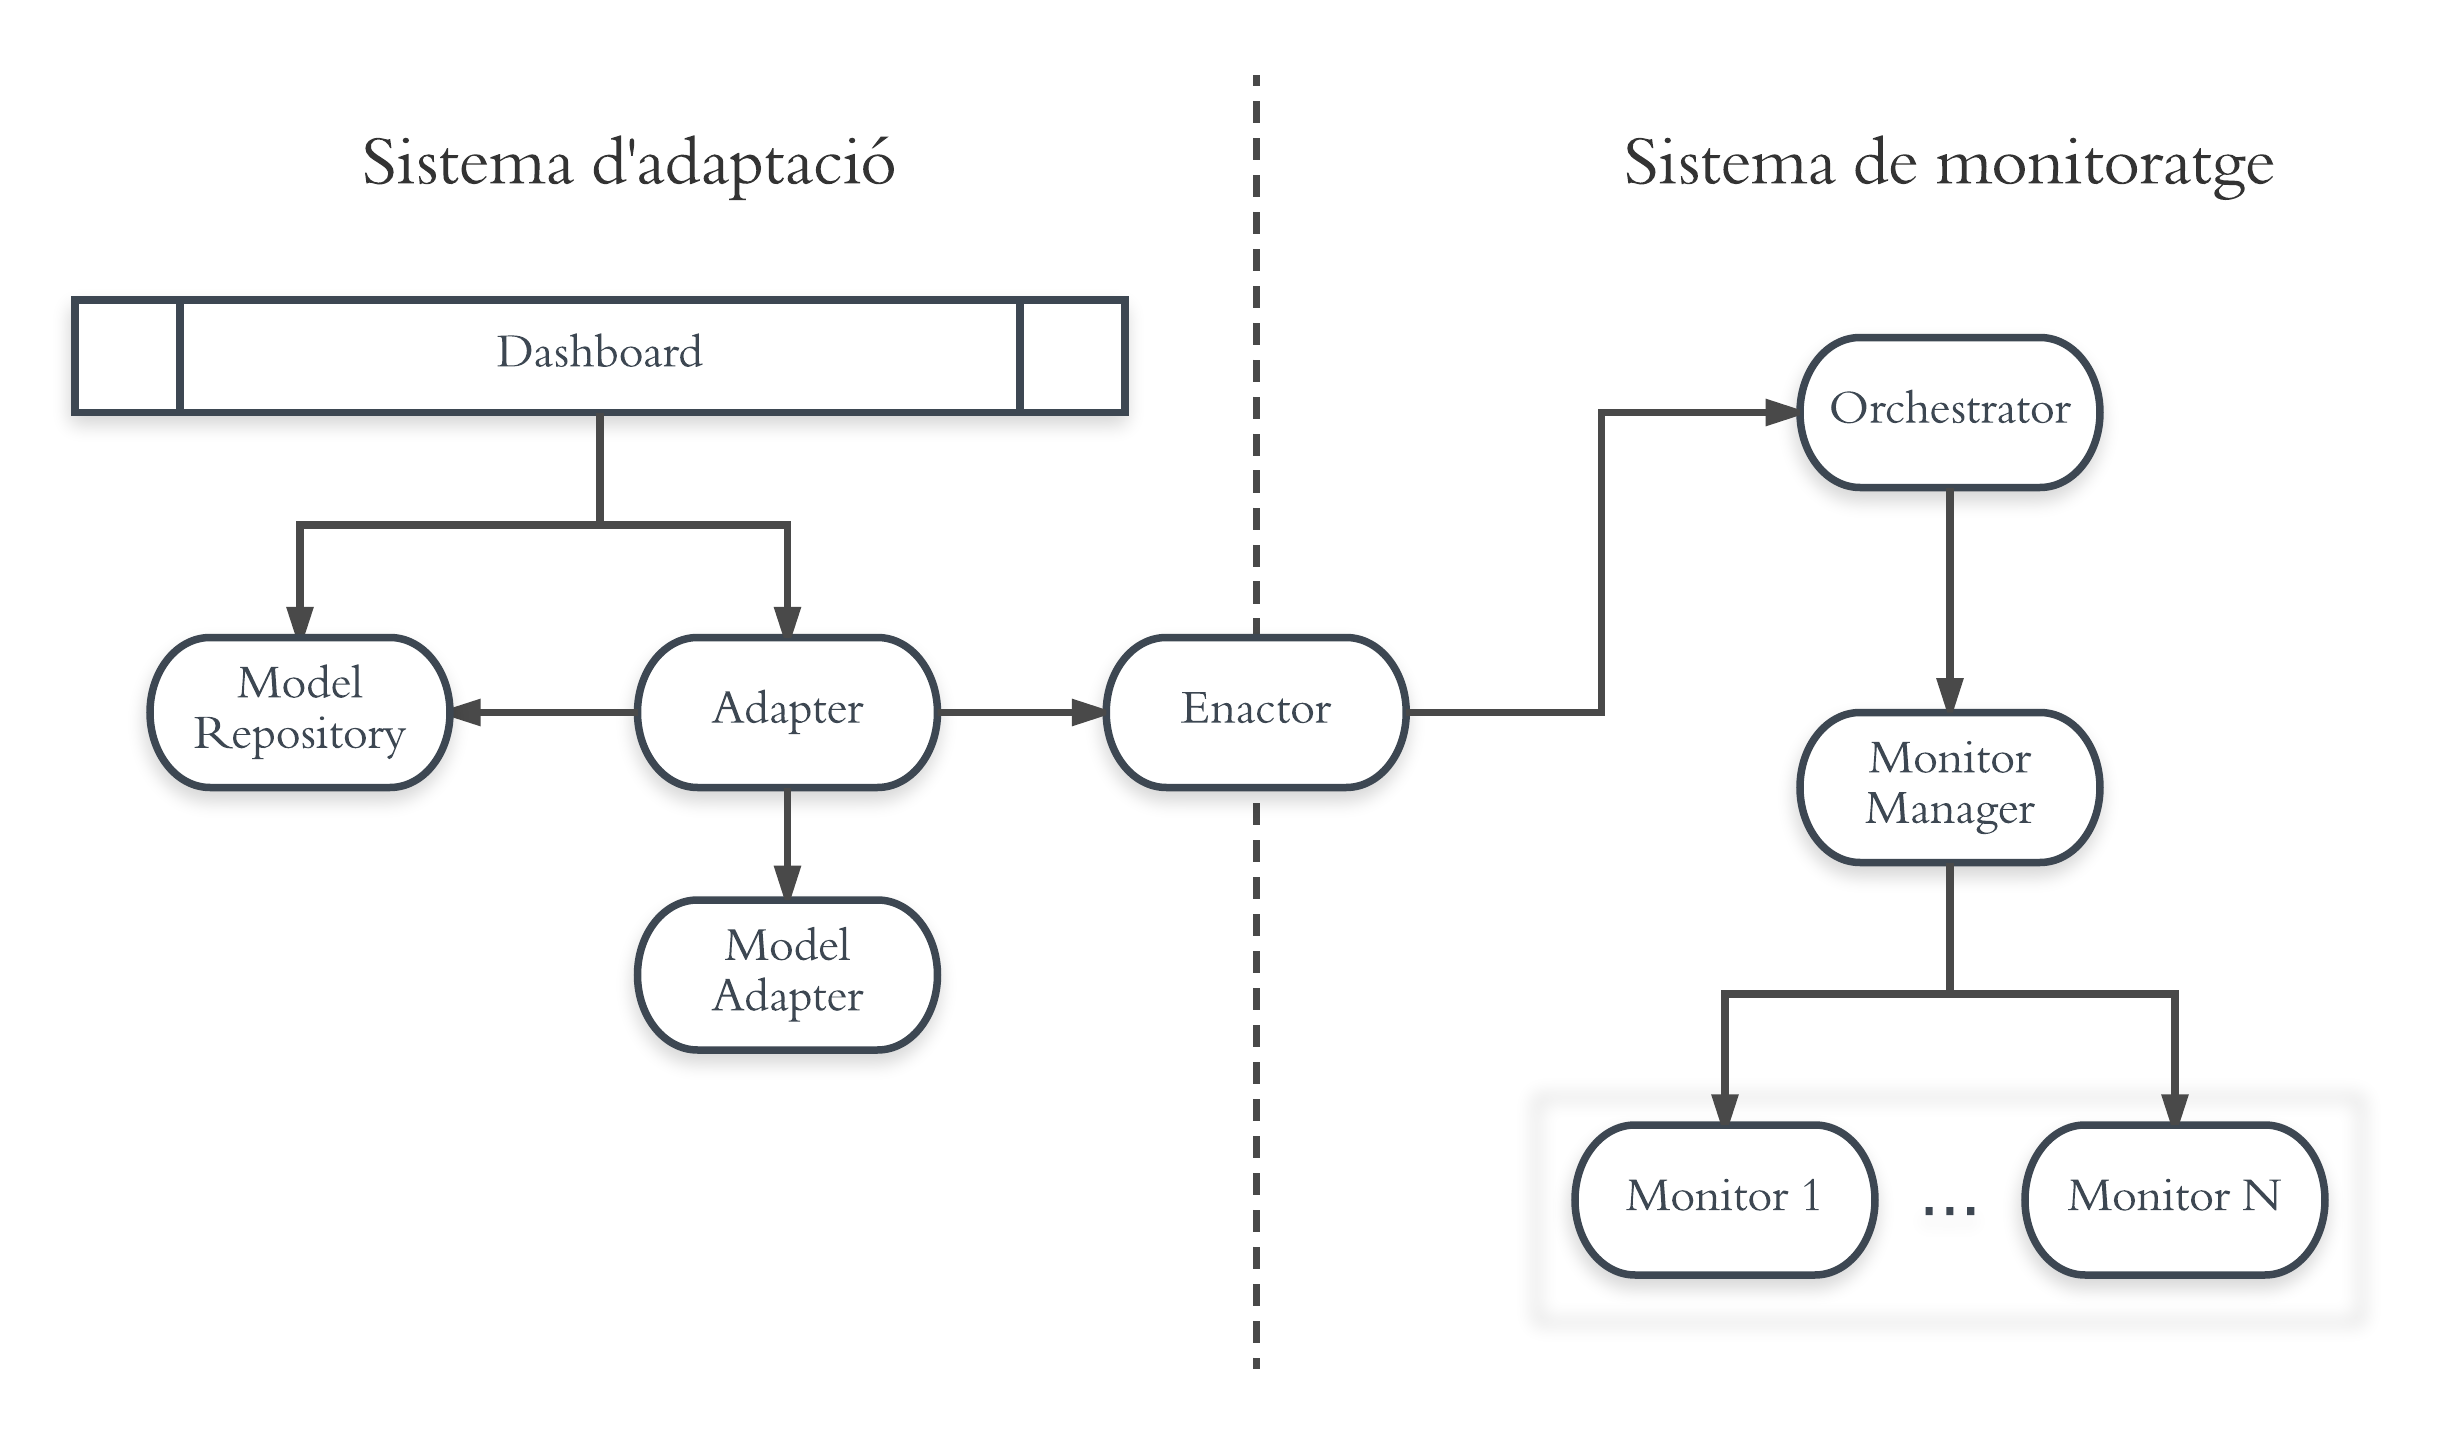
\includegraphics[width=13cm]{Figures/Figure4}
\decoRule
\caption[Disseny genèric del sistema proposat]{Disseny genèric del sistema proposat}
\label{fig:Figura4}
\end{figure}

\begin{itemize}
\item \textbf{Monitor.} Component de naturalesa ja descrita anteriorment, és l'encarregat de realitzar la col·lecció de dades d'un sistema software orientat al control de qualitat d'aquest. Dins el nostre sistema, disposarem d'un conjunt de monitors variats, conjunt que podrà ser extès sota diversos criteris i seguint el marc de la proposta de disseny plantejada.
\begin{itemize}
\item \textbf{\textit{Input}}. Informació/paràmetres de configuració d'un procés de monitoratge.
\item \textbf{\textit{Action}}. Procés de la informació per iniciar, aturar o modificar els paràmetres de la configuració d'un procés de monitoratge.
\item \textbf{\textit{Output}}. Conjunt de dades recol·lectades pels processos de monitoratge actius en el monitor.
\end{itemize}
\item \textbf{Monitor Manager.} Encarregat de gestionar l'activitat dels monitors, integrant el conjunt de monitors independents en el sistema sota un únic punt d'entrada, amb una semàntica genèrica. És l'encarregat, per tant, de redireccionar les diferents reconfiguracions (així com l'inici i aturada de processos de monitoratge) als monitors corresponents.
\begin{itemize}
\item \textbf{\textit{Input}}. Informació/paràmetres de configuració d'un procés de monitoratge per a un monitor específic.
\item \textbf{\textit{Action}}. Procés de la informació i transformació de la mateixa d'acord amb el monitor corresponent.
\item \textbf{\textit{Output}}. Informació/paràmetres de configuració transformats i orientats al monitor corresponent. 
\end{itemize}
\item \textbf{Orchestrator.} Aquest document forma part del context del projecte SUPERSEDE. Dins aquest projecte (presentat al capítol \textit{2.2.1. Projecte SUPERSEDE}), aquest component és el punt d'integració entre el subsistema d'adaptació de sistemes software i el subsistema de col·lecció i anàl·lisi de dades, i actua com a \textit{orquestrador} en un sentit de "pont" redireccional. En el marc del nostre projecte, que s'inclou a SUPERSEDE, aquest component actuarà com a punt entre el subsistema d'adaptació i el sistema de monitoratge
\begin{itemize}
\item \textbf{\textit{Input}}. Informació/paràmetres de configuració d'un procés de monitoratge per a un monitor específic.
\item \textbf{\textit{Action}}. Procés de la informació i transformació de la mateixa d'acord amb el propòsit del nostre sistema (configuració de monitors).
\item \textbf{\textit{Output}}. Informació/paràmetres de configuració transformats i orientats al sistema de monitoratge.
\end{itemize}
\end{itemize}

D'aquesta manera, el nostre sistema de monitoratge presenta 3 subcomponents independents que integren l'activitat de monitoratge mitjançant la comunicació entre ells: el sistema rep, a través de l'Orchestrator, peticions d'accions sobre els processos de monitoratge dels monitors. Aquest Orchestrator processa aquesta petició, i la redirecciona al Monitor Manager, qui coneix i controla els diferents monitors que hi ha al nostre sistema. El Monitor Manager s'encarrega d'analitzar la informació, processar-la d'acord al monitor al qual s'ha de redireccionar, i finalment enviar l'ordre de configuració al monitor corresponent. Amb aquesta informació ja processada per tal que el monitor concret pugui entendre-la, aquest adapta (és a dir, reconfigura) un procés de monitoratge existent, o bé en crea un de nou o n'elimina un d'existent, i procedeix amb el procés de monitoratge d'acord amb l'acció realitzada.\\

Definit els components del sistema de monitoratge, procedim a exposar els components i la interacció del \textbf{sistema d'adaptabilitat}:

\begin{itemize}
\item \textbf{Model Repository.} Aquest component s'encarrega de gestionar la persistència (lectura i escriptura) dels diferents models UML que defineixen les configuracions del nostre sistema de monitoratge. Els detalls d'aquests models UML, la seva sintaxi i el seu ús es descriuran més endavant.
\begin{itemize}
\item \textbf{\textit{Input}}. Peticions de lectura i escriptura dels models UML.
\item \textbf{\textit{Action}}. Accions pertinents sobre els models UML.
\item \textbf{\textit{Output}}. Retorna els models UML demanats d'acord amb la petició o modificació pertinent.
\end{itemize}
\item \textbf{Model Adapter.} Component que s'encarrega de realitzar adaptacions sobre els models UML que defineixen l'estat actual de les configuracions dels monitors d'acord amb les peticions d'adaptació que se li apliquen. Aquestes adaptacions sobre els diagrames definits s'apliquen en aquest component de forma aïllada, de manera que la resta del sistema no necessita tenir coneixement del procés tècnic de transformació dinàmica de models UML.
\begin{itemize}
\item \textbf{\textit{Input}}. Petició de modificació d'un model de configuració amb els models i paràmetres pertinents.
\item \textbf{\textit{Action}}. Modificació dinàmica del model UML d'acord amb la petició
\item \textbf{\textit{Output}}. Model UML transformat.
\end{itemize}
\item \textbf{Adapter.} És l'encarregat de realitzar l'adaptació del model des d'un punt de vista d'abstracció tècnica, centrant-se en la part semàntica de l'adaptació dels monitors. Mitjançant els models que defineixen el sistema i les possible millores, aquest component estudia i computa de forma automàtica reconfiguracions dels monitors.
\begin{itemize}
\item \textbf{\textit{Input}}. Lectura dels models del Model Repository per computar la petició d'adaptació de monitors.
\item \textbf{\textit{Action}}. Analitza els models i les possibles adaptacions per computar modificacions sobre els models de configuració, i demana aquesta modificació al Model Adapter.
\item \textbf{\textit{Output}}. Model/s de configuració adaptats.
\end{itemize}
\end{itemize}

En definitiva, el sistema d'adaptabilitat defineix un \textit{workflow} basat en una petició de reconfiguració a l'Adapter que, mitjançant l'anàlisi dels models que defineixen les configuracions dels monitors (configuracions actuals, propostes de noves configuracions, etc.) computa una modificació real sobre la configuració actual.\\

En aquest punt, necessitem un últim component que actui de pont entre el sistema d'adaptabilitat i el sistema de monitoratge, de tal manera que les adaptacions realitzades en el sistema d'adaptabilitat sobre els models UML que defineixen l'estat del sistema de monitoratge s'apliquin a aquest darrer. En aquest sentit, s'introdueix el component \textbf{Enactor.}

\begin{itemize}
\item \textbf{Enactor.} Component d'integració entre les adaptacions generades pel sistema i el sistema de monitoratge. Concretament, actua de pont entre l'Adapter, encarregat de gestionar aquestes reconfiguracions, i l'Orchestrator, component del sistema genèric a SUPERSEDE encarregat de gestionar totes les peticions d'adaptabilitat de components software. La seva tasca principal és afegir una capa d'abstracció entre els dos subsistemes, per evitar que aquests hagin de conèixer de l'activitat de l'altre.
\begin{itemize}
\item \textbf{\textit{Input}}. Model UML adaptat generat per l'Adapter amb una nova proposta de configuració del sistema.
\item \textbf{\textit{Action}}. Transformació del model UML en format processable per l'Orchestrator.
\item \textbf{\textit{Output}}. Petició de reconfiguració d'un monitor específic que envia a l'Orchestrator.
\end{itemize}
\end{itemize}

A termes genèrics, i sense entrar encara en detalls de disseny intern de cadascun d'aquests components, tenim una proposta inicial genèrica que defineix com ha de ser el nostre sistema, quins components l'han de formar i com s'han de relacionar entre ells per satisfer l'objectiu genèric d'aquest projecte.\\

Com a punt addicional, es proposa també el disseny d'un \textbf{dashboard} basat en una aplicació web senzilla, a través de la qual puguem visualitzar algunes de les dades de les adaptacions generades pel nostre sistema, amb l'objectiu de facilitar el control de l'activitat del sistema i la validació del mateix per una possible demostració.

\section{Integració de components}

La interacció entre els diferents components del sistema haurà de ser un dels elements a tractar en el desenvolupament del projecte. Un dels objectius principals és garantir el màxim desacoblament entre cadascuna d'aquestes interaccions, de tal manera que cadascun dels components puguin ser reaprofitats de forma independentment, i que a més la major part de modificacions en aquests components no afectin a la resta, com a mínim en termes d'interacció.\\

Per facilitar aquesta integració, el projecte SUPERSEDE ofereix una plataforma anomenada \textit{Integrated Framework} (IF), desenvolupada per un \textit{partner} del projecte. El seu objectiu és oferir una integració de tots els components desplegats al \textit{back-end} del sistema. A nivell tècnic, aquest component ofereix una llibreria amb un conjunt de \textit{proxies} implementats, a través dels quals els diferents components es poden comunicar amb altres components desplegats i afegits al IF.\\

Per permetre aquesta integració, l'únic requisit que planteja aquesta plataforma és l'exposició dels diferents components com a serveis web RESTful. D'aquesta manera, IF actua com a pont directe sense necessitat de formatar o "mapejar" els paràmetres d'entrada i sortida d'aquestes interaccions, ja que aquest component s'encarrega de fer les transformacions pertinents d'acord amb les necessitats d'interacció. \\

Veurem més endavant com aquest sistema aprofita aquest framework per facilitar la comunicació i evitar mapejats d'entrada/sortida. Amb aquest objectiu, serà necessari exposar alguns dels components com a serveis web.